\documentclass[]{article}
\usepackage{lmodern}
\usepackage{amssymb,amsmath}
\usepackage{ifxetex,ifluatex}
\usepackage{fixltx2e} % provides \textsubscript
\ifnum 0\ifxetex 1\fi\ifluatex 1\fi=0 % if pdftex
  \usepackage[T1]{fontenc}
  \usepackage[utf8]{inputenc}
\else % if luatex or xelatex
  \ifxetex
    \usepackage{mathspec}
  \else
    \usepackage{fontspec}
  \fi
  \defaultfontfeatures{Ligatures=TeX,Scale=MatchLowercase}
\fi
% use upquote if available, for straight quotes in verbatim environments
\IfFileExists{upquote.sty}{\usepackage{upquote}}{}
% use microtype if available
\IfFileExists{microtype.sty}{%
\usepackage{microtype}
\UseMicrotypeSet[protrusion]{basicmath} % disable protrusion for tt fonts
}{}
\usepackage[margin=1in]{geometry}
\usepackage{hyperref}
\hypersetup{unicode=true,
            pdfborder={0 0 0},
            breaklinks=true}
\urlstyle{same}  % don't use monospace font for urls
\usepackage{color}
\usepackage{fancyvrb}
\newcommand{\VerbBar}{|}
\newcommand{\VERB}{\Verb[commandchars=\\\{\}]}
\DefineVerbatimEnvironment{Highlighting}{Verbatim}{commandchars=\\\{\}}
% Add ',fontsize=\small' for more characters per line
\usepackage{framed}
\definecolor{shadecolor}{RGB}{248,248,248}
\newenvironment{Shaded}{\begin{snugshade}}{\end{snugshade}}
\newcommand{\AlertTok}[1]{\textcolor[rgb]{0.94,0.16,0.16}{#1}}
\newcommand{\AnnotationTok}[1]{\textcolor[rgb]{0.56,0.35,0.01}{\textbf{\textit{#1}}}}
\newcommand{\AttributeTok}[1]{\textcolor[rgb]{0.77,0.63,0.00}{#1}}
\newcommand{\BaseNTok}[1]{\textcolor[rgb]{0.00,0.00,0.81}{#1}}
\newcommand{\BuiltInTok}[1]{#1}
\newcommand{\CharTok}[1]{\textcolor[rgb]{0.31,0.60,0.02}{#1}}
\newcommand{\CommentTok}[1]{\textcolor[rgb]{0.56,0.35,0.01}{\textit{#1}}}
\newcommand{\CommentVarTok}[1]{\textcolor[rgb]{0.56,0.35,0.01}{\textbf{\textit{#1}}}}
\newcommand{\ConstantTok}[1]{\textcolor[rgb]{0.00,0.00,0.00}{#1}}
\newcommand{\ControlFlowTok}[1]{\textcolor[rgb]{0.13,0.29,0.53}{\textbf{#1}}}
\newcommand{\DataTypeTok}[1]{\textcolor[rgb]{0.13,0.29,0.53}{#1}}
\newcommand{\DecValTok}[1]{\textcolor[rgb]{0.00,0.00,0.81}{#1}}
\newcommand{\DocumentationTok}[1]{\textcolor[rgb]{0.56,0.35,0.01}{\textbf{\textit{#1}}}}
\newcommand{\ErrorTok}[1]{\textcolor[rgb]{0.64,0.00,0.00}{\textbf{#1}}}
\newcommand{\ExtensionTok}[1]{#1}
\newcommand{\FloatTok}[1]{\textcolor[rgb]{0.00,0.00,0.81}{#1}}
\newcommand{\FunctionTok}[1]{\textcolor[rgb]{0.00,0.00,0.00}{#1}}
\newcommand{\ImportTok}[1]{#1}
\newcommand{\InformationTok}[1]{\textcolor[rgb]{0.56,0.35,0.01}{\textbf{\textit{#1}}}}
\newcommand{\KeywordTok}[1]{\textcolor[rgb]{0.13,0.29,0.53}{\textbf{#1}}}
\newcommand{\NormalTok}[1]{#1}
\newcommand{\OperatorTok}[1]{\textcolor[rgb]{0.81,0.36,0.00}{\textbf{#1}}}
\newcommand{\OtherTok}[1]{\textcolor[rgb]{0.56,0.35,0.01}{#1}}
\newcommand{\PreprocessorTok}[1]{\textcolor[rgb]{0.56,0.35,0.01}{\textit{#1}}}
\newcommand{\RegionMarkerTok}[1]{#1}
\newcommand{\SpecialCharTok}[1]{\textcolor[rgb]{0.00,0.00,0.00}{#1}}
\newcommand{\SpecialStringTok}[1]{\textcolor[rgb]{0.31,0.60,0.02}{#1}}
\newcommand{\StringTok}[1]{\textcolor[rgb]{0.31,0.60,0.02}{#1}}
\newcommand{\VariableTok}[1]{\textcolor[rgb]{0.00,0.00,0.00}{#1}}
\newcommand{\VerbatimStringTok}[1]{\textcolor[rgb]{0.31,0.60,0.02}{#1}}
\newcommand{\WarningTok}[1]{\textcolor[rgb]{0.56,0.35,0.01}{\textbf{\textit{#1}}}}
\usepackage{graphicx,grffile}
\makeatletter
\def\maxwidth{\ifdim\Gin@nat@width>\linewidth\linewidth\else\Gin@nat@width\fi}
\def\maxheight{\ifdim\Gin@nat@height>\textheight\textheight\else\Gin@nat@height\fi}
\makeatother
% Scale images if necessary, so that they will not overflow the page
% margins by default, and it is still possible to overwrite the defaults
% using explicit options in \includegraphics[width, height, ...]{}
\setkeys{Gin}{width=\maxwidth,height=\maxheight,keepaspectratio}
\IfFileExists{parskip.sty}{%
\usepackage{parskip}
}{% else
\setlength{\parindent}{0pt}
\setlength{\parskip}{6pt plus 2pt minus 1pt}
}
\setlength{\emergencystretch}{3em}  % prevent overfull lines
\providecommand{\tightlist}{%
  \setlength{\itemsep}{0pt}\setlength{\parskip}{0pt}}
\setcounter{secnumdepth}{0}
% Redefines (sub)paragraphs to behave more like sections
\ifx\paragraph\undefined\else
\let\oldparagraph\paragraph
\renewcommand{\paragraph}[1]{\oldparagraph{#1}\mbox{}}
\fi
\ifx\subparagraph\undefined\else
\let\oldsubparagraph\subparagraph
\renewcommand{\subparagraph}[1]{\oldsubparagraph{#1}\mbox{}}
\fi

%%% Use protect on footnotes to avoid problems with footnotes in titles
\let\rmarkdownfootnote\footnote%
\def\footnote{\protect\rmarkdownfootnote}

%%% Change title format to be more compact
\usepackage{titling}

% Create subtitle command for use in maketitle
\providecommand{\subtitle}[1]{
  \posttitle{
    \begin{center}\large#1\end{center}
    }
}

\setlength{\droptitle}{-2em}

  \title{}
    \pretitle{\vspace{\droptitle}}
  \posttitle{}
    \author{}
    \preauthor{}\postauthor{}
    \date{}
    \predate{}\postdate{}
  

\begin{document}

\hypertarget{examen-parcial---caso-airfares}{%
\section{Examen Parcial - Caso
Airfares}\label{examen-parcial---caso-airfares}}

La industria de las aerolíneas es un sector de rápido crecimiento,
altamente competitivo y sujeto a cambios drásticos, incluso pequeños
cambios en algunos parámetros críticos.~Por lo tanto, aplicar el proceso
de minería de datos a la toma de decisiones es muy crítico para una
supervivencia y éxito más prolongados.~Nuestro objetivo principal es
implementar un modelo para una de las principales aerolíneas de los EE.
UU., Para determinar si necesitan comenzar a operar hacia / desde los
aeropuertos recientemente abiertos y cómo deberían fijar el precio de
los vuelos en estas nuevas rutas.~El análisis se basó en los datos
históricos recopilados de una aerolínea en 638 rutas aéreas en los
Estados Unidos.

\begin{Shaded}
\begin{Highlighting}[]
\FunctionTok{library}\NormalTok{(}\StringTok{\textquotesingle{}dplyr\textquotesingle{}}\NormalTok{) }\CommentTok{\# Funciones sencillas para realizar manipulación de datos en R}
\end{Highlighting}
\end{Shaded}

\begin{verbatim}
## Warning: package 'dplyr' was built under R version 3.6.3
\end{verbatim}

\begin{verbatim}
## 
## Attaching package: 'dplyr'
\end{verbatim}

\begin{verbatim}
## The following objects are masked from 'package:stats':
## 
##     filter, lag
\end{verbatim}

\begin{verbatim}
## The following objects are masked from 'package:base':
## 
##     intersect, setdiff, setequal, union
\end{verbatim}

\begin{Shaded}
\begin{Highlighting}[]
\FunctionTok{library}\NormalTok{(}\StringTok{\textquotesingle{}corrplot\textquotesingle{}}\NormalTok{) }\CommentTok{\# Contiene varias funciones de utilidad básicos que incluyen: funciones estadísticas, de lectura / escritura, muestras, etc}
\end{Highlighting}
\end{Shaded}

\begin{verbatim}
## corrplot 0.92 loaded
\end{verbatim}

\begin{Shaded}
\begin{Highlighting}[]
\FunctionTok{library}\NormalTok{(}\StringTok{\textquotesingle{}caTools\textquotesingle{}}\NormalTok{) }\CommentTok{\# Visualización de datos en R}
\FunctionTok{library}\NormalTok{(}\StringTok{\textquotesingle{}ggplot2\textquotesingle{}}\NormalTok{) }\CommentTok{\# Para trazar una matriz de correlación que muestre la relación entre cada variable.}
\end{Highlighting}
\end{Shaded}

\begin{verbatim}
## Registered S3 methods overwritten by 'ggplot2':
##   method         from 
##   [.quosures     rlang
##   c.quosures     rlang
##   print.quosures rlang
\end{verbatim}

\begin{Shaded}
\begin{Highlighting}[]
\FunctionTok{library}\NormalTok{(}\StringTok{\textquotesingle{}caret\textquotesingle{}}\NormalTok{) }\CommentTok{\# Creación de variables ficticias para este caso.}
\end{Highlighting}
\end{Shaded}

\begin{verbatim}
## Loading required package: lattice
\end{verbatim}

\begin{Shaded}
\begin{Highlighting}[]
\FunctionTok{library}\NormalTok{(}\StringTok{\textquotesingle{}rpart\textquotesingle{}}\NormalTok{) }\CommentTok{\# Se utiliza para crear modelos de árbol basados en regresión.}
\FunctionTok{library}\NormalTok{(}\StringTok{\textquotesingle{}xgboost\textquotesingle{}}\NormalTok{) }\CommentTok{\# Se utiliza para crear modelos de impulso recién entrenados que aprenden de series anteriores de modelos y son eficientes, flexibles y portátiles}
\end{Highlighting}
\end{Shaded}

\begin{verbatim}
## Warning: package 'xgboost' was built under R version 3.6.3
\end{verbatim}

\begin{verbatim}
## 
## Attaching package: 'xgboost'
\end{verbatim}

\begin{verbatim}
## The following object is masked from 'package:dplyr':
## 
##     slice
\end{verbatim}

\begin{Shaded}
\begin{Highlighting}[]
\FunctionTok{library}\NormalTok{(}\StringTok{\textquotesingle{}glmnet\textquotesingle{}}\NormalTok{) }\CommentTok{\# Se adapta a modelos lineales / modelos lineales generalizados que penalizan la probabilidad máxima, con regresión LASSO / Ridge}
\end{Highlighting}
\end{Shaded}

\begin{verbatim}
## Warning: package 'glmnet' was built under R version 3.6.3
\end{verbatim}

\begin{verbatim}
## Loading required package: Matrix
\end{verbatim}

\begin{verbatim}
## Loaded glmnet 4.1-1
\end{verbatim}

\begin{Shaded}
\begin{Highlighting}[]
\FunctionTok{sessionInfo}\NormalTok{()}
\end{Highlighting}
\end{Shaded}

\begin{verbatim}
## R version 3.6.1 (2019-07-05)
## Platform: x86_64-w64-mingw32/x64 (64-bit)
## Running under: Windows 10 x64 (build 19043)
## 
## Matrix products: default
## 
## locale:
## [1] LC_COLLATE=Spanish_Peru.1252  LC_CTYPE=Spanish_Peru.1252   
## [3] LC_MONETARY=Spanish_Peru.1252 LC_NUMERIC=C                 
## [5] LC_TIME=Spanish_Peru.1252    
## 
## attached base packages:
## [1] stats     graphics  grDevices utils     datasets  methods   base     
## 
## other attached packages:
##  [1] glmnet_4.1-1     Matrix_1.2-17    xgboost_1.4.1.1  rpart_4.1-15    
##  [5] caret_6.0-83     lattice_0.20-38  ggplot2_3.1.1    caTools_1.17.1.2
##  [9] corrplot_0.92    dplyr_1.0.6     
## 
## loaded via a namespace (and not attached):
##  [1] shape_1.4.6        tidyselect_1.1.1   xfun_0.6          
##  [4] reshape2_1.4.3     purrr_0.3.2        splines_3.6.1     
##  [7] colorspace_1.4-1   vctrs_0.3.8        generics_0.1.1    
## [10] stats4_3.6.1       htmltools_0.3.6    yaml_2.2.0        
## [13] prodlim_2018.04.18 utf8_1.1.4         survival_2.44-1.1 
## [16] rlang_0.4.11       ModelMetrics_1.2.2 pillar_1.6.4      
## [19] glue_1.4.2         withr_2.4.3        DBI_1.0.0         
## [22] foreach_1.4.4      lifecycle_1.0.1    plyr_1.8.4        
## [25] lava_1.6.5         stringr_1.4.0      timeDate_3043.102 
## [28] munsell_0.5.0      gtable_0.3.0       recipes_0.1.5     
## [31] codetools_0.2-16   evaluate_0.13      knitr_1.22        
## [34] class_7.3-15       fansi_0.4.0        Rcpp_1.0.1        
## [37] scales_1.0.0       ipred_0.9-8        jsonlite_1.6      
## [40] digest_0.6.18      stringi_1.4.3      grid_3.6.1        
## [43] tools_3.6.1        bitops_1.0-6       magrittr_2.0.1    
## [46] lazyeval_0.2.2     tibble_3.1.1       crayon_1.3.4      
## [49] pkgconfig_2.0.2    ellipsis_0.3.2     MASS_7.3-51.3     
## [52] data.table_1.12.2  lubridate_1.7.4    gower_0.2.0       
## [55] rmarkdown_1.12     iterators_1.0.10   R6_2.4.0          
## [58] nnet_7.3-12        nlme_3.1-139       compiler_3.6.1
\end{verbatim}

\begin{Shaded}
\begin{Highlighting}[]
\NormalTok{Airfare.data }\OtherTok{=}  \FunctionTok{read.csv}\NormalTok{(}\StringTok{"Data.csv"}\NormalTok{)}
\NormalTok{Airfare.data }\OtherTok{=}\NormalTok{ Airfare.data[,}\SpecialCharTok{{-}}\DecValTok{19}\NormalTok{]}


\FunctionTok{dim}\NormalTok{(Airfare.data)  }\CommentTok{\#638  18, meaning 638 rows and 18 columns}
\end{Highlighting}
\end{Shaded}

\begin{verbatim}
## [1] 638  18
\end{verbatim}

\begin{Shaded}
\begin{Highlighting}[]
\FunctionTok{str}\NormalTok{(Airfare.data)}
\end{Highlighting}
\end{Shaded}

\begin{verbatim}
## 'data.frame':    638 obs. of  18 variables:
##  $ S_CODE  : Factor w/ 8 levels "*","DCA","EWR",..: 1 1 1 8 7 1 1 1 1 1 ...
##  $ S_CITY  : Factor w/ 51 levels "Albuquerque         NM",..: 14 3 7 9 9 11 14 18 23 25 ...
##  $ E_CODE  : Factor w/ 8 levels "*","DCA","EWR",..: 1 1 1 1 1 1 1 1 1 1 ...
##  $ E_CITY  : Factor w/ 68 levels "Amarillo            TX",..: 1 2 2 2 2 2 2 2 2 2 ...
##  $ COUPON  : num  1 1.06 1.06 1.06 1.06 1.01 1.28 1.15 1.33 1.6 ...
##  $ NEW     : int  3 3 3 3 3 3 3 3 3 2 ...
##  $ VACATION: Factor w/ 2 levels "No","Yes": 1 1 1 1 1 1 1 2 1 1 ...
##  $ SW      : Factor w/ 2 levels "No","Yes": 2 1 1 2 2 2 1 2 2 2 ...
##  $ HI      : num  5292 5419 9185 2657 2657 ...
##  $ S_INCOME: Factor w/ 50 levels "$14,600","$18,933",..: 37 34 44 41 41 29 37 33 35 26 ...
##  $ E_INCOME: Factor w/ 67 levels "$14,600","$18,851",..: 7 57 57 57 57 57 57 57 57 57 ...
##  $ S_POP   : int  3036732 3532657 5787293 7830332 7830332 2230955 3036732 1440377 3770125 1694803 ...
##  $ E_POP   : int  205711 7145897 7145897 7145897 7145897 7145897 7145897 7145897 7145897 7145897 ...
##  $ SLOT    : Factor w/ 2 levels "Controlled","Free": 2 2 2 1 2 2 2 2 2 2 ...
##  $ GATE    : Factor w/ 2 levels "Constrained",..: 2 2 2 2 2 2 2 2 2 2 ...
##  $ DISTANCE: int  312 576 364 612 612 309 1220 921 1249 964 ...
##  $ PAX     : int  7864 8820 6452 25144 25144 13386 4625 5512 7811 4657 ...
##  $ FARE    : Factor w/ 451 levels "$100.36","$100.80",..: 371 170 219 427 427 345 241 48 168 41 ...
\end{verbatim}

\begin{Shaded}
\begin{Highlighting}[]
\NormalTok{Airfare.data}\SpecialCharTok{$}\NormalTok{FARE }\OtherTok{=} \FunctionTok{as.numeric}\NormalTok{(}\FunctionTok{substr}\NormalTok{(}\FunctionTok{as.character}\NormalTok{(Airfare.data}\SpecialCharTok{$}\NormalTok{FARE),}\DecValTok{2}\NormalTok{,}\DecValTok{10}\NormalTok{)) }\CommentTok{\# To remove currency $}

\DocumentationTok{\#\# S\_INCOME AND E\_INCOME are factors, we will need to convert it into number, and remove currency symbol}

\NormalTok{Airfare.data}\SpecialCharTok{$}\NormalTok{S\_INCOME }\OtherTok{=} \FunctionTok{as.numeric}\NormalTok{(}\FunctionTok{gsub}\NormalTok{(}\StringTok{"}\SpecialCharTok{\textbackslash{}\textbackslash{}}\StringTok{$|,"}\NormalTok{,}\StringTok{""}\NormalTok{,Airfare.data}\SpecialCharTok{$}\NormalTok{S\_INCOME))}
\NormalTok{Airfare.data}\SpecialCharTok{$}\NormalTok{E\_INCOME }\OtherTok{=} \FunctionTok{as.numeric}\NormalTok{(}\FunctionTok{gsub}\NormalTok{(}\StringTok{"}\SpecialCharTok{\textbackslash{}\textbackslash{}}\StringTok{$|,"}\NormalTok{,}\StringTok{""}\NormalTok{,Airfare.data}\SpecialCharTok{$}\NormalTok{E\_INCOME))}

\NormalTok{Airfare }\OtherTok{=}\NormalTok{ Airfare.data[,}\DecValTok{5}\SpecialCharTok{:}\DecValTok{18}\NormalTok{]                   }\CommentTok{\# Removing the unwanted columns that have text values}

\FunctionTok{dim}\NormalTok{(Airfare)      }\CommentTok{\# Getting the dimension ( no of rows and columns in our data)}
\end{Highlighting}
\end{Shaded}

\begin{verbatim}
## [1] 638  14
\end{verbatim}

\begin{Shaded}
\begin{Highlighting}[]
\FunctionTok{summary}\NormalTok{(Airfare)   }\CommentTok{\# Summary of data}
\end{Highlighting}
\end{Shaded}

\begin{verbatim}
##      COUPON           NEW        VACATION    SW            HI       
##  Min.   :1.000   Min.   :0.000   No :468   No :444   Min.   : 1230  
##  1st Qu.:1.040   1st Qu.:3.000   Yes:170   Yes:194   1st Qu.: 3090  
##  Median :1.150   Median :3.000                       Median : 4208  
##  Mean   :1.202   Mean   :2.754                       Mean   : 4442  
##  3rd Qu.:1.298   3rd Qu.:3.000                       3rd Qu.: 5481  
##  Max.   :1.940   Max.   :3.000                       Max.   :10000  
##     S_INCOME        E_INCOME         S_POP             E_POP        
##  Min.   :14600   Min.   :14600   Min.   :  29838   Min.   : 111745  
##  1st Qu.:24706   1st Qu.:23903   1st Qu.:1862106   1st Qu.:1228816  
##  Median :28637   Median :26409   Median :3532657   Median :2195215  
##  Mean   :27760   Mean   :27664   Mean   :4557004   Mean   :3194503  
##  3rd Qu.:29694   3rd Qu.:31981   3rd Qu.:7830332   3rd Qu.:4549784  
##  Max.   :38813   Max.   :38813   Max.   :9056076   Max.   :9056076  
##          SLOT              GATE        DISTANCE           PAX       
##  Controlled:182   Constrained:124   Min.   : 114.0   Min.   : 1504  
##  Free      :456   Free       :514   1st Qu.: 455.0   1st Qu.: 5328  
##                                     Median : 850.0   Median : 7792  
##                                     Mean   : 975.7   Mean   :12782  
##                                     3rd Qu.:1306.2   3rd Qu.:14090  
##                                     Max.   :2764.0   Max.   :73892  
##       FARE       
##  Min.   : 42.47  
##  1st Qu.:106.29  
##  Median :144.60  
##  Mean   :160.88  
##  3rd Qu.:209.35  
##  Max.   :402.02
\end{verbatim}

\begin{Shaded}
\begin{Highlighting}[]
\NormalTok{Airfare.corr }\OtherTok{=} \FunctionTok{select\_if}\NormalTok{(Airfare, is.numeric) }\CommentTok{\# selecting the one which are numeric}
\NormalTok{coorelation }\OtherTok{=} \FunctionTok{corrplot}\NormalTok{(}\FunctionTok{cor}\NormalTok{(Airfare.corr), }\AttributeTok{type =} \StringTok{"upper"}\NormalTok{, }\AttributeTok{method =} \StringTok{"number"}\NormalTok{)}
\end{Highlighting}
\end{Shaded}

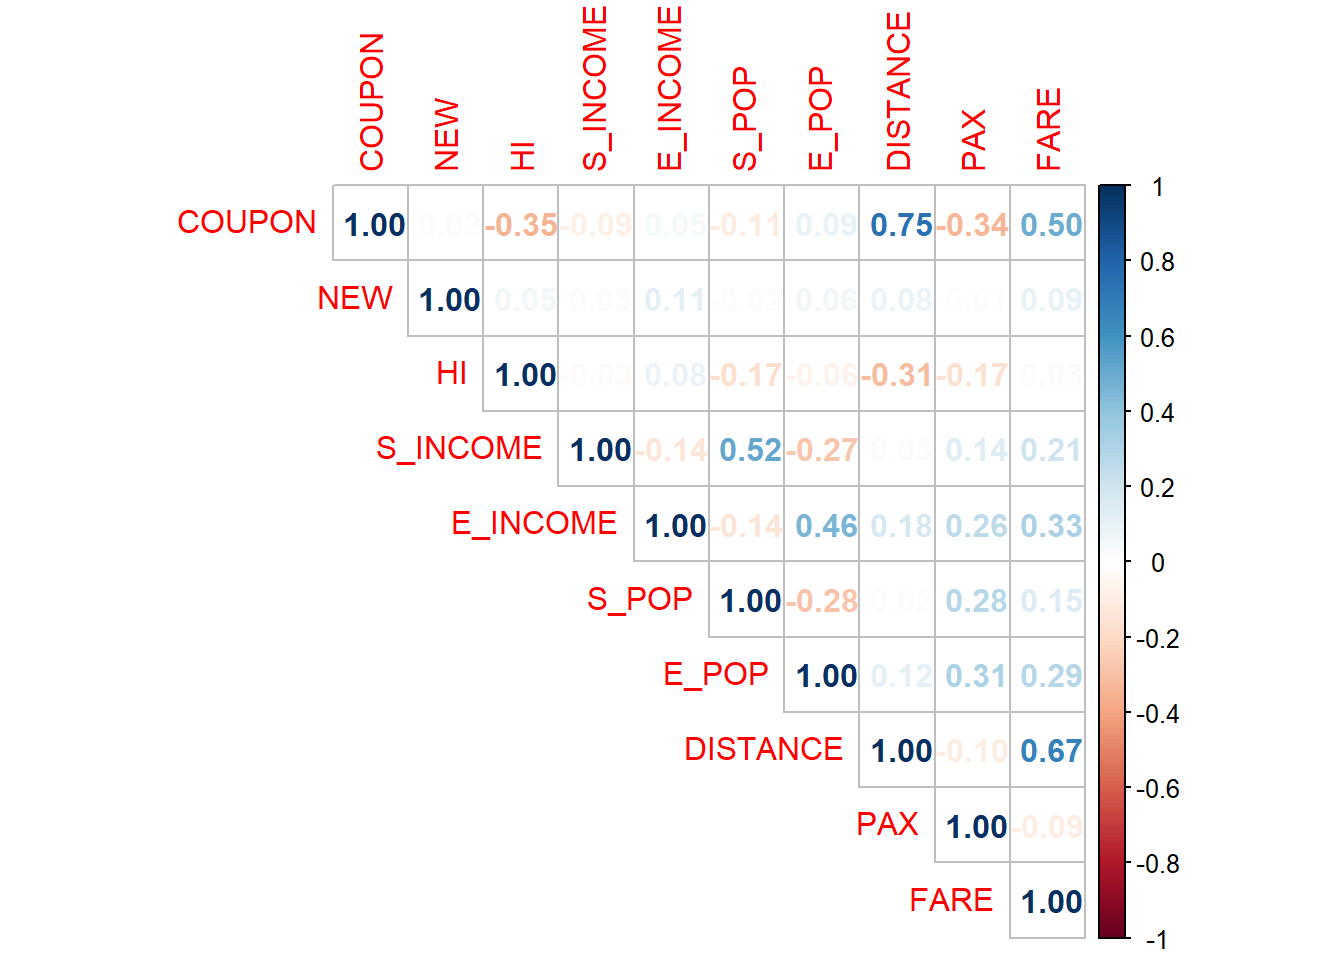
\includegraphics{Airfares_files/figure-latex/unnamed-chunk-7-1.pdf}

\begin{Shaded}
\begin{Highlighting}[]
\FunctionTok{plot}\NormalTok{(}\AttributeTok{x =}\NormalTok{ Airfare}\SpecialCharTok{$}\NormalTok{DISTANCE, }\AttributeTok{y =}\NormalTok{ Airfare}\SpecialCharTok{$}\NormalTok{FARE,}\AttributeTok{type =} \StringTok{"p"}\NormalTok{, }\AttributeTok{main =} \StringTok{"Relation between Distance and Fair"}\NormalTok{, }\AttributeTok{xlab =} \StringTok{"Dist between 2 airports"}\NormalTok{, }\AttributeTok{ylab =} \StringTok{"Avg Price"}\NormalTok{)}
\end{Highlighting}
\end{Shaded}

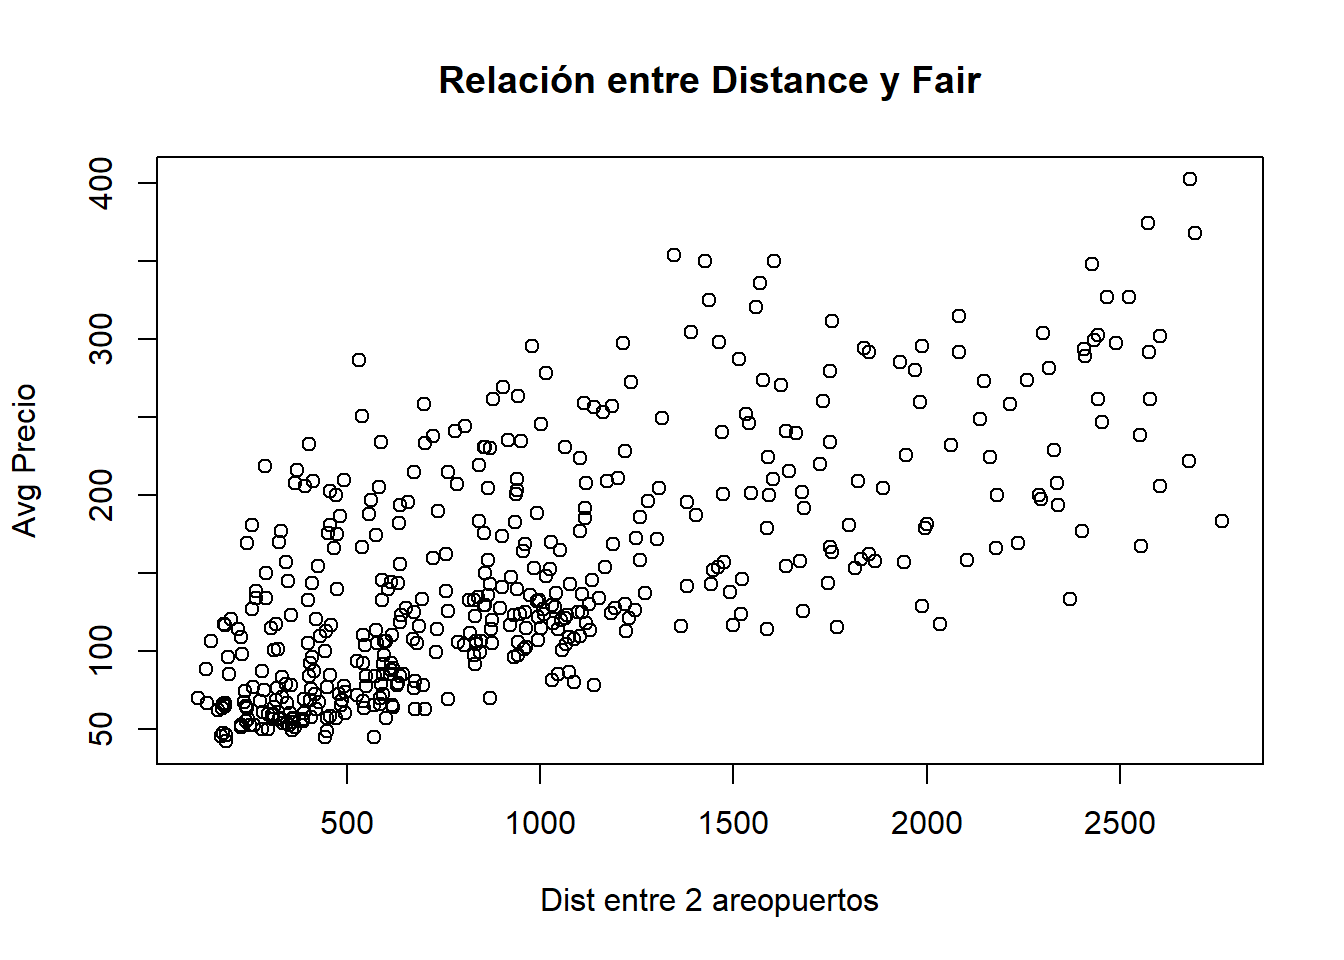
\includegraphics{Airfares_files/figure-latex/unnamed-chunk-8-1.pdf}

\begin{Shaded}
\begin{Highlighting}[]
\FunctionTok{plot}\NormalTok{(}\AttributeTok{x =}\NormalTok{ Airfare}\SpecialCharTok{$}\NormalTok{COUPON, }\AttributeTok{y =}\NormalTok{ Airfare}\SpecialCharTok{$}\NormalTok{FARE,}\AttributeTok{type =} \StringTok{"p"}\NormalTok{, }\AttributeTok{main =} \StringTok{"Relation between No of Flights Stops and respective Fair"}\NormalTok{, }\AttributeTok{xlab =} \StringTok{"No of Flights Stops"}\NormalTok{, }\AttributeTok{ylab =} \StringTok{"Avg Price"}\NormalTok{)}
\end{Highlighting}
\end{Shaded}

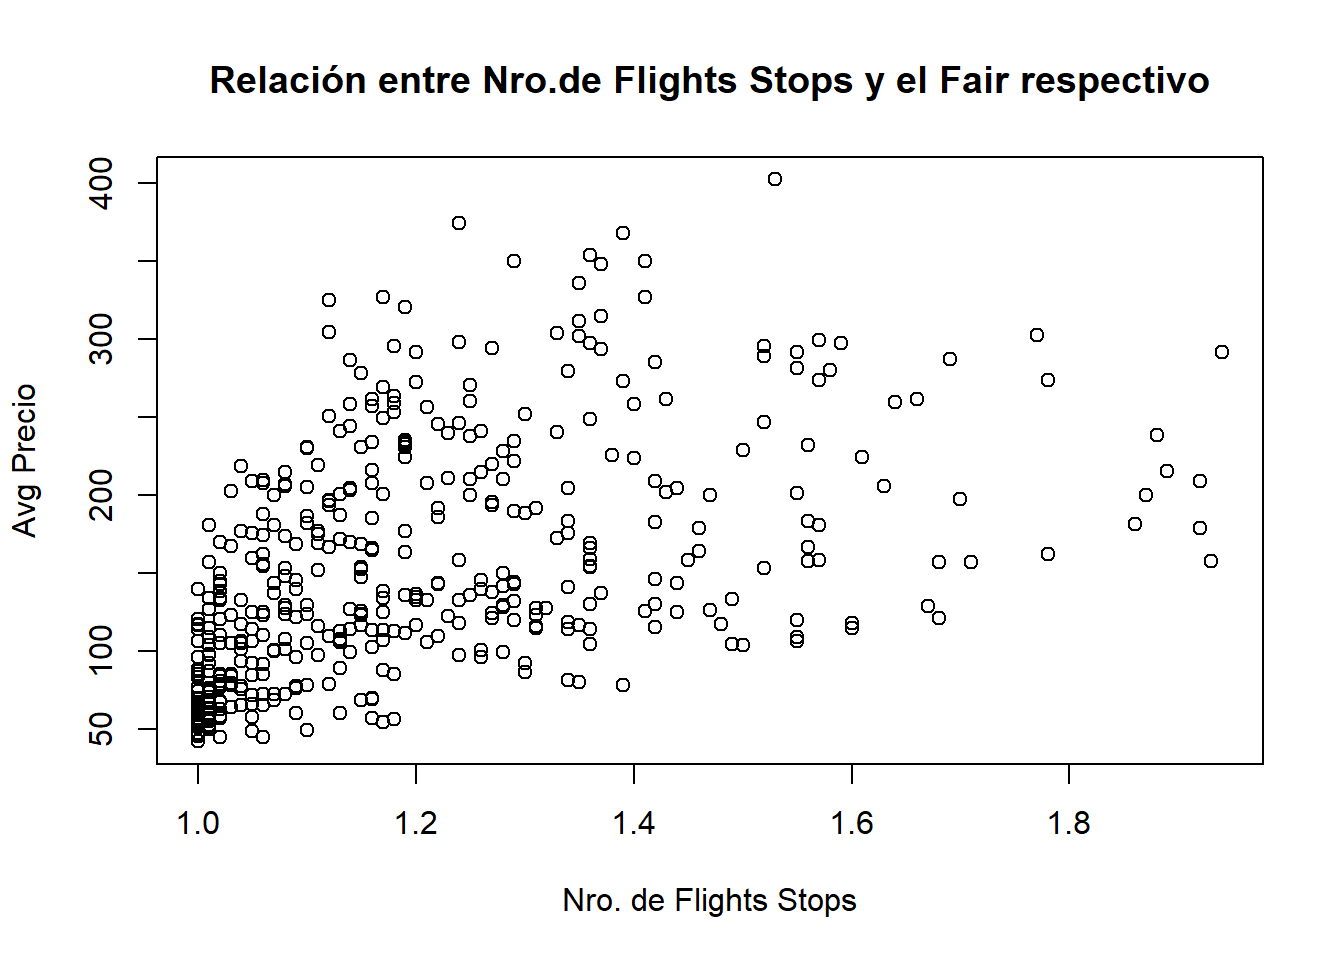
\includegraphics{Airfares_files/figure-latex/unnamed-chunk-9-1.pdf}

\begin{Shaded}
\begin{Highlighting}[]
\CommentTok{\#install.packages("caret", dependencies = c("Depends", "Suggests"))}

\CommentTok{\# converting dummy variables}
\NormalTok{DummyVar }\OtherTok{=} \FunctionTok{dummyVars}\NormalTok{(}\StringTok{"\textasciitilde{}."}\NormalTok{,}\AttributeTok{data =}\NormalTok{ Airfare)}
\NormalTok{Airfare }\OtherTok{=} \FunctionTok{data.frame}\NormalTok{(}\FunctionTok{predict}\NormalTok{(DummyVar, }\AttributeTok{newdata =}\NormalTok{ Airfare))}

\DocumentationTok{\#\# FEAUTURE SCALING}
\NormalTok{Airfare[,}\SpecialCharTok{{-}}\DecValTok{18}\NormalTok{] }\OtherTok{\textless{}{-}} \FunctionTok{lapply}\NormalTok{(Airfare[,}\SpecialCharTok{{-}}\DecValTok{18}\NormalTok{], }\ControlFlowTok{function}\NormalTok{(x) }\ControlFlowTok{if}\NormalTok{(}\FunctionTok{is.numeric}\NormalTok{(x))\{(x }\SpecialCharTok{{-}} \FunctionTok{min}\NormalTok{(x))}\SpecialCharTok{/}\NormalTok{(}\FunctionTok{max}\NormalTok{(x) }\SpecialCharTok{{-}} \FunctionTok{min}\NormalTok{(x))\} }\ControlFlowTok{else}\NormalTok{ x)}

\CommentTok{\# SPLITTING DATA INTO TRAINING AND }\AlertTok{TESTING}\CommentTok{ SETS}
\NormalTok{sampleSplit }\OtherTok{=} \FunctionTok{sample.split}\NormalTok{(Airfare,}\AttributeTok{SplitRatio =} \FloatTok{0.8}\NormalTok{)}
\NormalTok{Airfare.training }\OtherTok{=} \FunctionTok{subset}\NormalTok{(Airfare, sampleSplit }\SpecialCharTok{==} \ConstantTok{TRUE}\NormalTok{)}
\NormalTok{Airfare.test }\OtherTok{=} \FunctionTok{subset}\NormalTok{(Airfare, sampleSplit }\SpecialCharTok{==} \ConstantTok{FALSE}\NormalTok{)}
\end{Highlighting}
\end{Shaded}

Multiple linear regresion

\begin{Shaded}
\begin{Highlighting}[]
\FunctionTok{set.seed}\NormalTok{(}\DecValTok{100}\NormalTok{)}
\NormalTok{modelLr }\OtherTok{=} \FunctionTok{lm}\NormalTok{(FARE }\SpecialCharTok{\textasciitilde{}}\NormalTok{., }\AttributeTok{data =}\NormalTok{ Airfare.training)}
\FunctionTok{summary}\NormalTok{(modelLr)}
\end{Highlighting}
\end{Shaded}

\begin{verbatim}
## 
## Call:
## lm(formula = FARE ~ ., data = Airfare.training)
## 
## Residuals:
##      Min       1Q   Median       3Q      Max 
## -102.932  -23.281   -1.692   23.063  104.507 
## 
## Coefficients: (4 not defined because of singularities)
##                    Estimate Std. Error t value Pr(>|t|)    
## (Intercept)      -4.828e+01  1.137e+01  -4.247 2.60e-05 ***
## COUPON            5.861e-04  1.285e+01   0.000 0.999964    
## NEW              -2.138e+00  6.625e+00  -0.323 0.747038    
## VACATION.No       3.516e+01  4.199e+00   8.374 6.13e-16 ***
## VACATION.Yes             NA         NA      NA       NA    
## SW.No             3.949e+01  4.323e+00   9.134  < 2e-16 ***
## SW.Yes                   NA         NA      NA       NA    
## HI                7.844e+01  9.864e+00   7.952 1.31e-14 ***
## S_INCOME          2.296e+01  1.446e+01   1.588 0.112851    
## E_INCOME          4.868e+01  1.045e+01   4.660 4.11e-06 ***
## S_POP             3.375e+01  6.854e+00   4.924 1.17e-06 ***
## E_POP             3.118e+01  7.735e+00   4.031 6.44e-05 ***
## SLOT.Controlled   1.657e+01  4.445e+00   3.728 0.000216 ***
## SLOT.Free                NA         NA      NA       NA    
## GATE.Constrained  2.217e+01  4.514e+00   4.911 1.24e-06 ***
## GATE.Free                NA         NA      NA       NA    
## DISTANCE          1.976e+02  1.074e+01  18.391  < 2e-16 ***
## PAX              -6.399e+01  1.209e+01  -5.294 1.82e-07 ***
## ---
## Signif. codes:  0 '***' 0.001 '**' 0.01 '*' 0.05 '.' 0.1 ' ' 1
## 
## Residual standard error: 35.8 on 482 degrees of freedom
## Multiple R-squared:  0.7832, Adjusted R-squared:  0.7773 
## F-statistic: 133.9 on 13 and 482 DF,  p-value: < 2.2e-16
\end{verbatim}

\begin{Shaded}
\begin{Highlighting}[]
\FunctionTok{set.seed}\NormalTok{(}\DecValTok{100}\NormalTok{)}
\NormalTok{modelLR }\OtherTok{=} \FunctionTok{lm}\NormalTok{(FARE }\SpecialCharTok{\textasciitilde{}}\NormalTok{ VACATION.No}\SpecialCharTok{+}\NormalTok{SW.No}\SpecialCharTok{+}\NormalTok{HI}\SpecialCharTok{+}\NormalTok{E\_INCOME}\SpecialCharTok{+}\NormalTok{S\_POP}\SpecialCharTok{+}\NormalTok{E\_POP}\SpecialCharTok{+}\NormalTok{SLOT.Controlled}\SpecialCharTok{+}\NormalTok{GATE.Constrained}\SpecialCharTok{+}\NormalTok{DISTANCE}\SpecialCharTok{+}\NormalTok{PAX, }\AttributeTok{data =}\NormalTok{ Airfare.training)}
\NormalTok{LR.predict }\OtherTok{=} \FunctionTok{predict}\NormalTok{(modelLR, }\AttributeTok{newdata =}\NormalTok{ Airfare.test[,}\SpecialCharTok{{-}}\DecValTok{18}\NormalTok{])}

\DocumentationTok{\#\# Calculating Mean Squared Error}
\NormalTok{AccuracyLR }\OtherTok{=} \FunctionTok{sum}\NormalTok{(}\FunctionTok{abs}\NormalTok{(LR.predict }\SpecialCharTok{{-}}\NormalTok{ Airfare.test[,}\DecValTok{18}\NormalTok{]))}\SpecialCharTok{/}\FunctionTok{length}\NormalTok{(Airfare.test[,}\DecValTok{18}\NormalTok{])}

\DocumentationTok{\#\# Plotting the graph}
\FunctionTok{plot}\NormalTok{(modelLR)}
\end{Highlighting}
\end{Shaded}

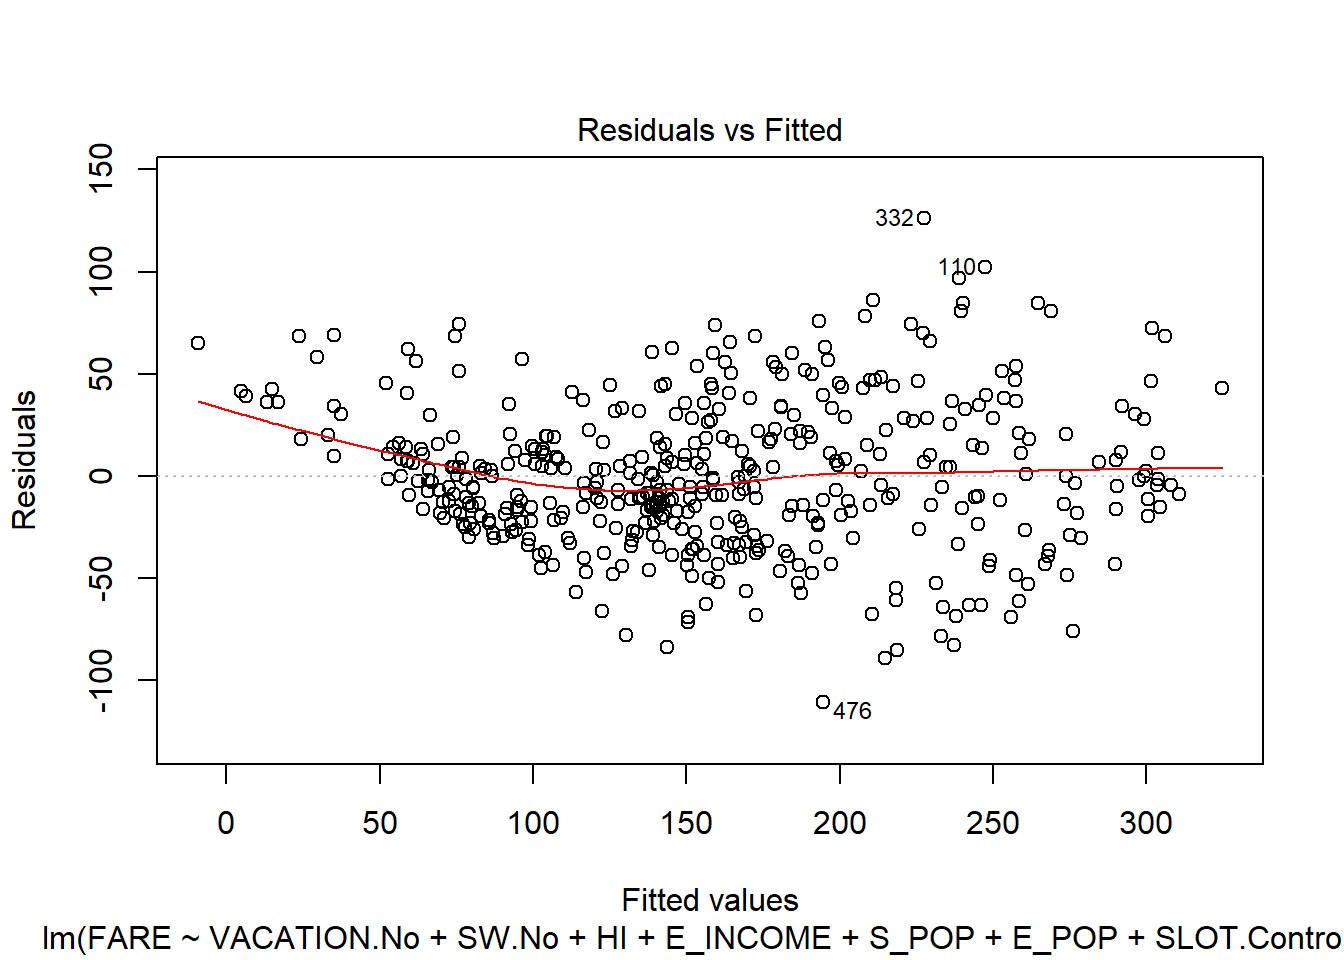
\includegraphics{Airfares_files/figure-latex/unnamed-chunk-12-1.pdf}
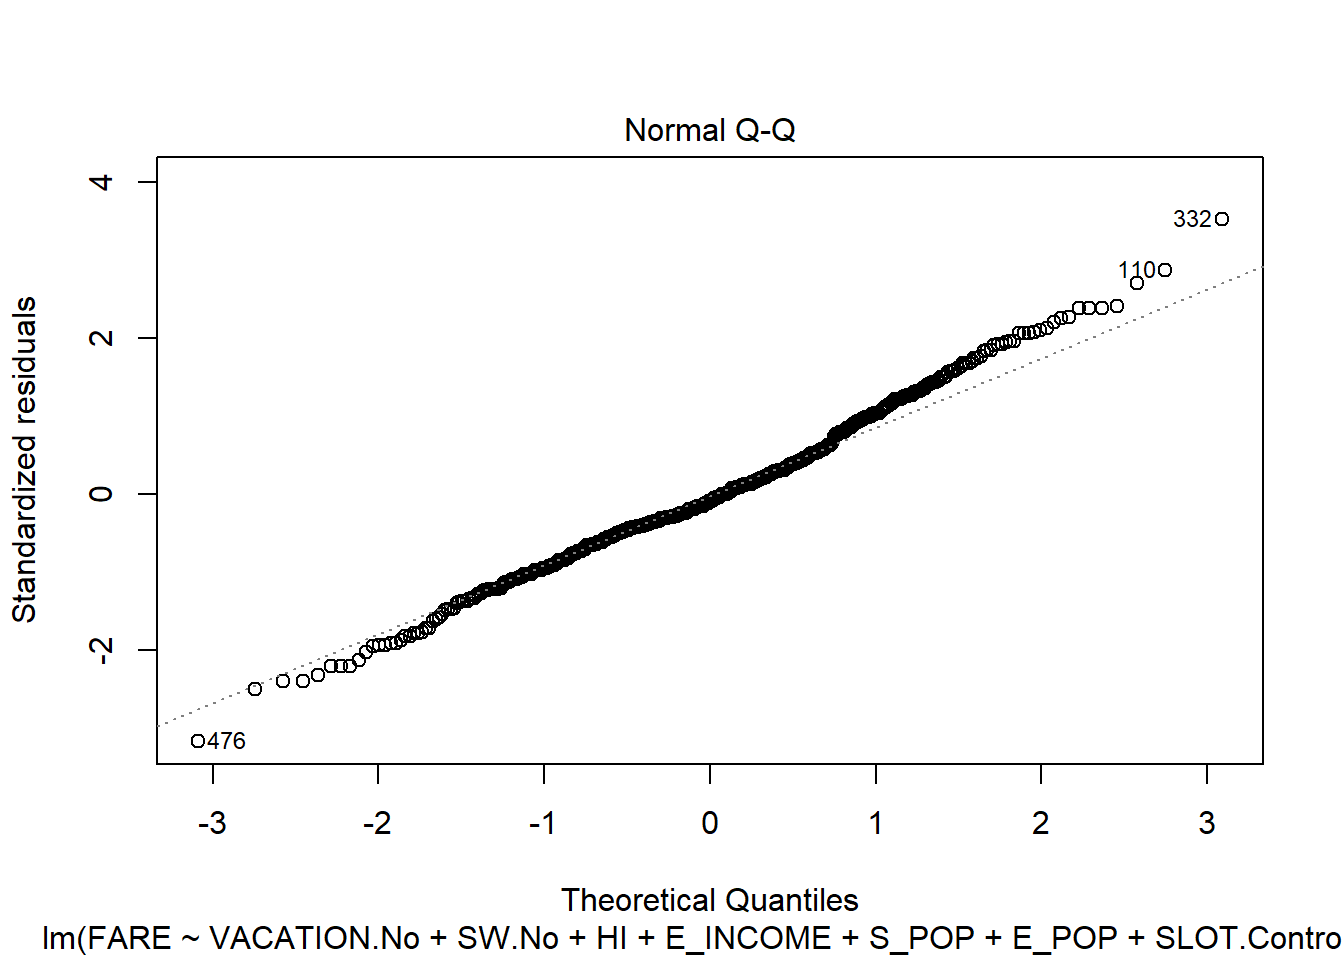
\includegraphics{Airfares_files/figure-latex/unnamed-chunk-12-2.pdf}
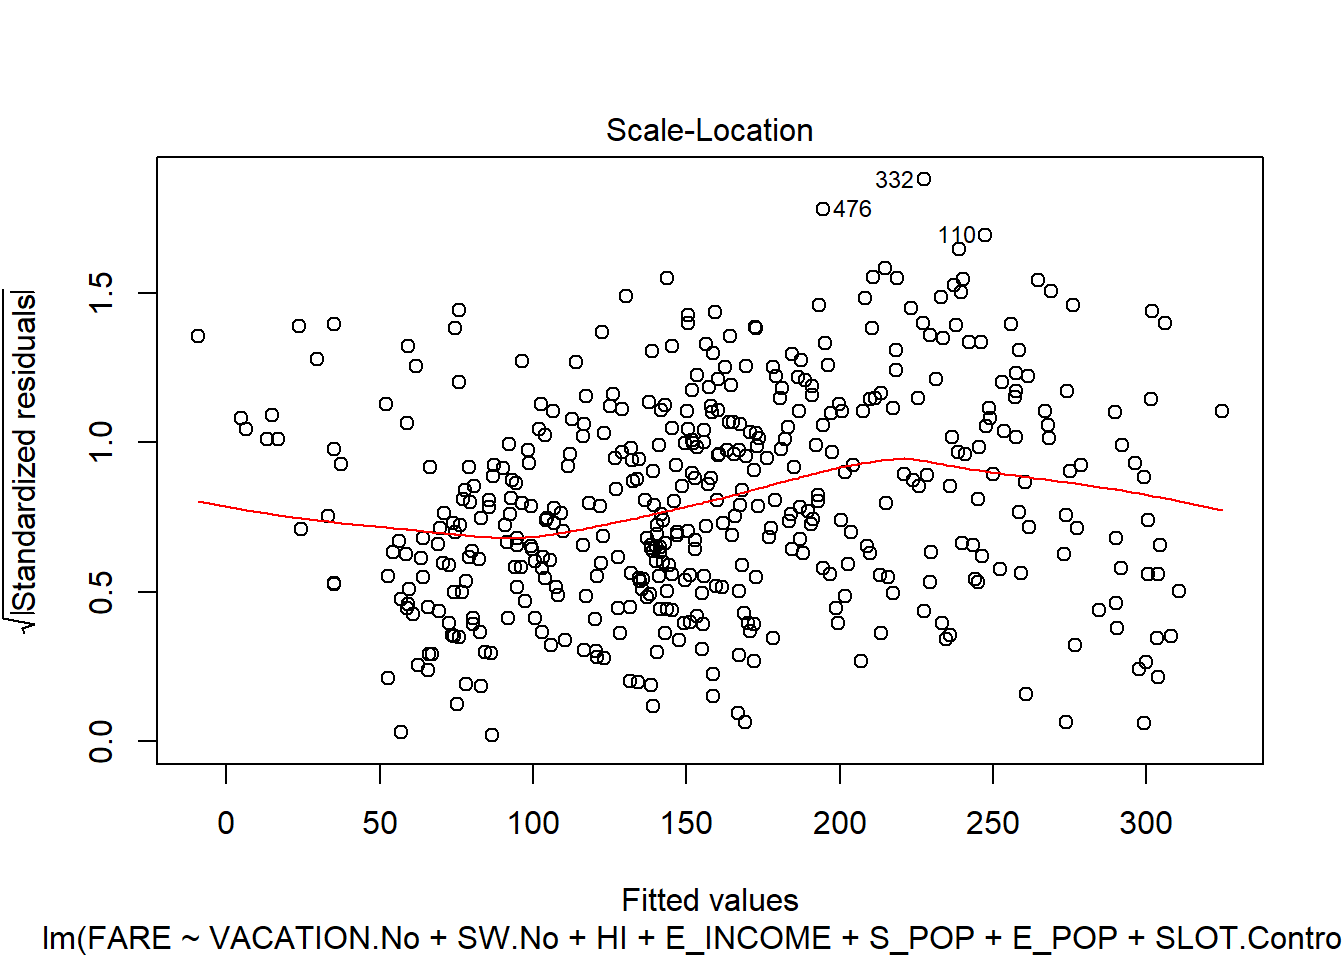
\includegraphics{Airfares_files/figure-latex/unnamed-chunk-12-3.pdf}
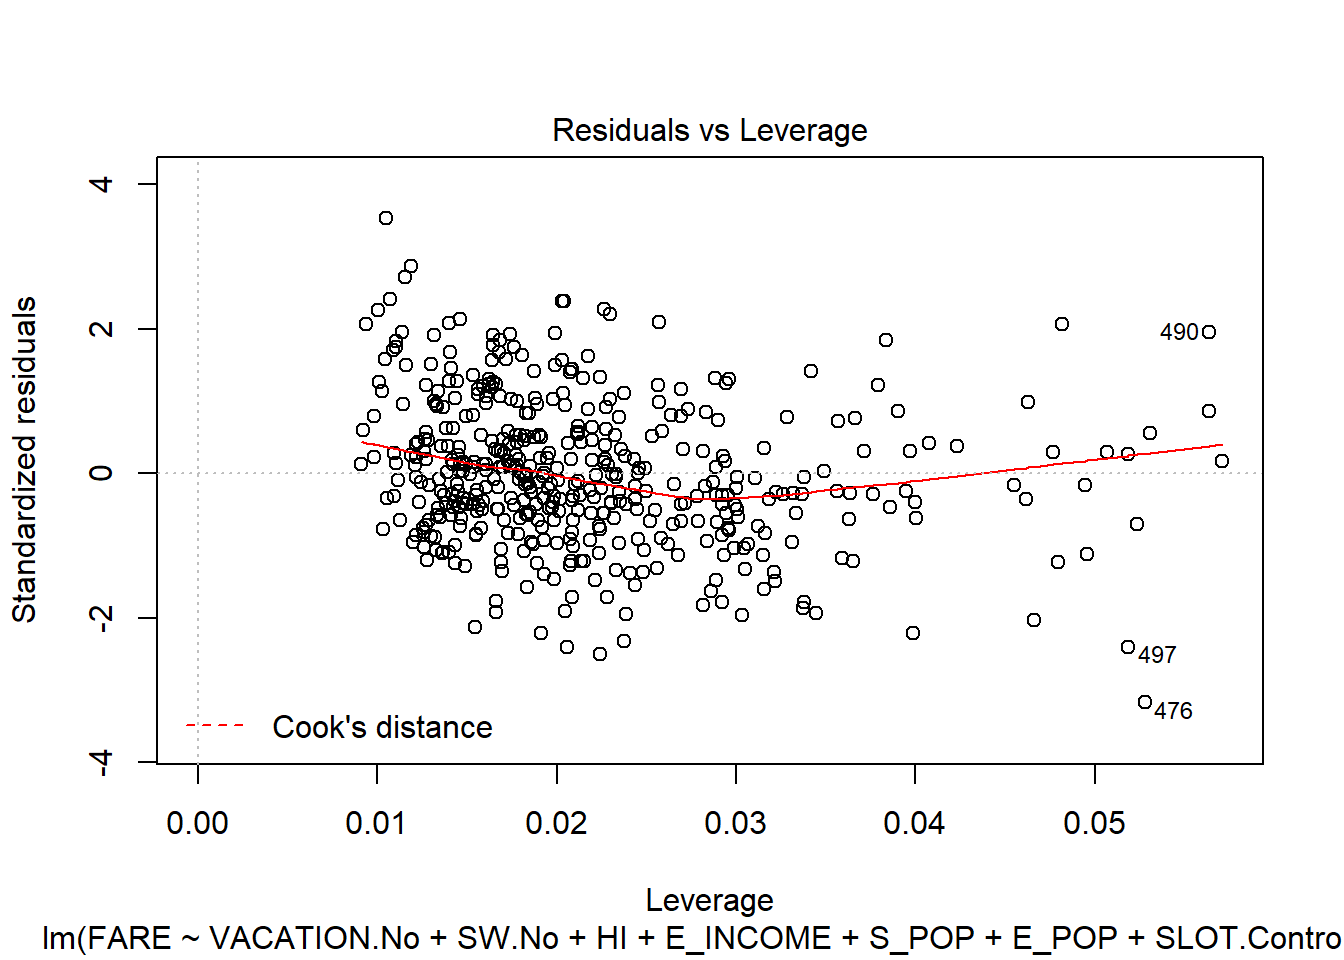
\includegraphics{Airfares_files/figure-latex/unnamed-chunk-12-4.pdf}

desicion tree model

\begin{Shaded}
\begin{Highlighting}[]
\FunctionTok{set.seed}\NormalTok{(}\DecValTok{100}\NormalTok{)}
\NormalTok{modelDT }\OtherTok{=} \FunctionTok{rpart}\NormalTok{(FARE }\SpecialCharTok{\textasciitilde{}}\NormalTok{.,}\AttributeTok{data =}\NormalTok{ Airfare.training)}
\NormalTok{DT.Predict }\OtherTok{=} \FunctionTok{predict}\NormalTok{(modelDT, }\AttributeTok{newdata =}\NormalTok{ Airfare.test[,}\SpecialCharTok{{-}}\DecValTok{18}\NormalTok{])}

\DocumentationTok{\#\# Calculating Mean Squared Error       }
\NormalTok{AccuracyDT }\OtherTok{=} \FunctionTok{sum}\NormalTok{(}\FunctionTok{abs}\NormalTok{(DT.Predict }\SpecialCharTok{{-}}\NormalTok{ Airfare.test[,}\DecValTok{18}\NormalTok{]))}\SpecialCharTok{/}\FunctionTok{length}\NormalTok{(Airfare.test[,}\DecValTok{18}\NormalTok{]) }
\end{Highlighting}
\end{Shaded}

extreme gradient boosting

\begin{Shaded}
\begin{Highlighting}[]
\FunctionTok{set.seed}\NormalTok{(}\DecValTok{100}\NormalTok{)}

\NormalTok{lab\_matrix }\OtherTok{=} \FunctionTok{as.matrix}\NormalTok{(Airfare.training}\SpecialCharTok{$}\NormalTok{FARE)}
\NormalTok{data\_trainX }\OtherTok{=} \FunctionTok{as.matrix}\NormalTok{(Airfare.training[,}\SpecialCharTok{{-}}\DecValTok{18}\NormalTok{])}
\NormalTok{dtrain }\OtherTok{=} \FunctionTok{xgb.DMatrix}\NormalTok{(}\AttributeTok{data =}\NormalTok{ data\_trainX, }\AttributeTok{label =}\NormalTok{ lab\_matrix)}
\FunctionTok{dim}\NormalTok{(}\FunctionTok{as.matrix}\NormalTok{(Airfare.training}\SpecialCharTok{$}\NormalTok{FARE))}
\end{Highlighting}
\end{Shaded}

\begin{verbatim}
## [1] 496   1
\end{verbatim}

\begin{Shaded}
\begin{Highlighting}[]
\NormalTok{dtest }\OtherTok{=} \FunctionTok{xgb.DMatrix}\NormalTok{(}\AttributeTok{data =} \FunctionTok{as.matrix}\NormalTok{(Airfare.test[,}\SpecialCharTok{{-}}\DecValTok{18}\NormalTok{]), }\AttributeTok{label =} \FunctionTok{as.matrix}\NormalTok{(Airfare.test}\SpecialCharTok{$}\NormalTok{FARE))}

\CommentTok{\# Defining the parameters}
\NormalTok{parameters }\OtherTok{=} \FunctionTok{list}\NormalTok{(}\AttributeTok{booster =} \StringTok{"gblinear"}\NormalTok{,}
                  \AttributeTok{objective =} \StringTok{"reg:linear"}\NormalTok{,    }
                  \AttributeTok{eta =} \FloatTok{0.1}\NormalTok{,           }\CommentTok{\#Vary btwn 0.1{-}0.3}
                  \AttributeTok{nthread =} \DecValTok{5}\NormalTok{,         }\CommentTok{\#Increase this to improve speed}
                  \AttributeTok{max\_depth =} \DecValTok{15}\NormalTok{,}
                  \AttributeTok{lambda=} \FloatTok{0.5}\NormalTok{,         }\CommentTok{\#Vary between 0{-}3}
                  \AttributeTok{alpha=} \FloatTok{0.5}\NormalTok{,          }\CommentTok{\#Vary between 0{-}3}
                  \AttributeTok{min\_child\_weight=} \DecValTok{2}\NormalTok{, }\CommentTok{\#Vary btwn 1{-}10}
                  \AttributeTok{eval\_metric =} \StringTok{"rmse"}\NormalTok{)}

\NormalTok{model.Xgb }\OtherTok{=} \FunctionTok{xgboost}\NormalTok{(}\AttributeTok{params =}\NormalTok{ parameters, }\AttributeTok{data =}\NormalTok{ dtrain, }\AttributeTok{nrounds =} \DecValTok{53}\NormalTok{)}
\end{Highlighting}
\end{Shaded}

\begin{verbatim}
## [23:45:48] WARNING: amalgamation/../src/objective/regression_obj.cu:171: reg:linear is now deprecated in favor of reg:squarederror.
## [23:45:48] WARNING: amalgamation/../src/learner.cc:573: 
## Parameters: { "max_depth", "min_child_weight" } might not be used.
## 
##   This may not be accurate due to some parameters are only used in language bindings but
##   passed down to XGBoost core.  Or some parameters are not used but slip through this
##   verification. Please open an issue if you find above cases.
## 
## 
## [1]  train-rmse:115.428925 
## [2]  train-rmse:85.982361 
## [3]  train-rmse:73.209824 
## [4]  train-rmse:67.613113 
## [5]  train-rmse:64.904053 
## [6]  train-rmse:63.388531 
## [7]  train-rmse:62.426342 
## [8]  train-rmse:61.739380 
## [9]  train-rmse:61.209824 
## [10] train-rmse:60.782532 
## [11] train-rmse:60.420124 
## [12] train-rmse:60.114044 
## [13] train-rmse:59.853649 
## [14] train-rmse:59.636829 
## [15] train-rmse:59.436726 
## [16] train-rmse:59.268078 
## [17] train-rmse:59.124367 
## [18] train-rmse:58.991875 
## [19] train-rmse:58.874268 
## [20] train-rmse:58.774601 
## [21] train-rmse:58.688183 
## [22] train-rmse:58.611877 
## [23] train-rmse:58.546272 
## [24] train-rmse:58.484055 
## [25] train-rmse:58.429482 
## [26] train-rmse:58.382370 
## [27] train-rmse:58.342350 
## [28] train-rmse:58.305111 
## [29] train-rmse:58.276085 
## [30] train-rmse:58.248753 
## [31] train-rmse:58.226227 
## [32] train-rmse:58.204849 
## [33] train-rmse:58.188690 
## [34] train-rmse:58.172634 
## [35] train-rmse:58.162106 
## [36] train-rmse:58.154308 
## [37] train-rmse:58.147167 
## [38] train-rmse:58.139801 
## [39] train-rmse:58.135258 
## [40] train-rmse:58.132423 
## [41] train-rmse:58.131535 
## [42] train-rmse:58.129623 
## [43] train-rmse:58.130592 
## [44] train-rmse:58.131001 
## [45] train-rmse:58.133293 
## [46] train-rmse:58.139069 
## [47] train-rmse:58.143127 
## [48] train-rmse:58.147648 
## [49] train-rmse:58.153606 
## [50] train-rmse:58.158104 
## [51] train-rmse:58.164177 
## [52] train-rmse:58.168453 
## [53] train-rmse:58.174053
\end{verbatim}

\begin{Shaded}
\begin{Highlighting}[]
\NormalTok{model.Predict }\OtherTok{=} \FunctionTok{predict}\NormalTok{(model.Xgb, dtest)}

\NormalTok{AccuracyXgb }\OtherTok{=} \FunctionTok{sum}\NormalTok{(}\FunctionTok{abs}\NormalTok{(model.Predict }\SpecialCharTok{{-}}\NormalTok{ Airfare.test[,}\DecValTok{18}\NormalTok{]))}\SpecialCharTok{/}\FunctionTok{length}\NormalTok{(Airfare.test[,}\DecValTok{18}\NormalTok{]) }
\end{Highlighting}
\end{Shaded}

\begin{Shaded}
\begin{Highlighting}[]
\FunctionTok{set.seed}\NormalTok{(}\DecValTok{100}\NormalTok{)}
\CommentTok{\# The input must be a matrix in case of LASSO}
\NormalTok{Airfare\_X }\OtherTok{=} \FunctionTok{as.matrix}\NormalTok{(Airfare[,}\SpecialCharTok{{-}}\DecValTok{18}\NormalTok{])}
\NormalTok{Airfare\_Y }\OtherTok{=}\NormalTok{ Airfare}\SpecialCharTok{$}\NormalTok{FARE}
\NormalTok{lasso\_fit }\OtherTok{=} \FunctionTok{glmnet}\NormalTok{(}\AttributeTok{x =}\NormalTok{ Airfare\_X, }\AttributeTok{y =}\NormalTok{ Airfare\_Y,}\AttributeTok{family =}\StringTok{"gaussian"}\NormalTok{,}\AttributeTok{alpha =} \DecValTok{1}\NormalTok{ )}

\FunctionTok{plot}\NormalTok{(lasso\_fit, }\AttributeTok{xvar =} \StringTok{"lambda"}\NormalTok{, }\AttributeTok{label =} \ConstantTok{TRUE}\NormalTok{)}
\end{Highlighting}
\end{Shaded}

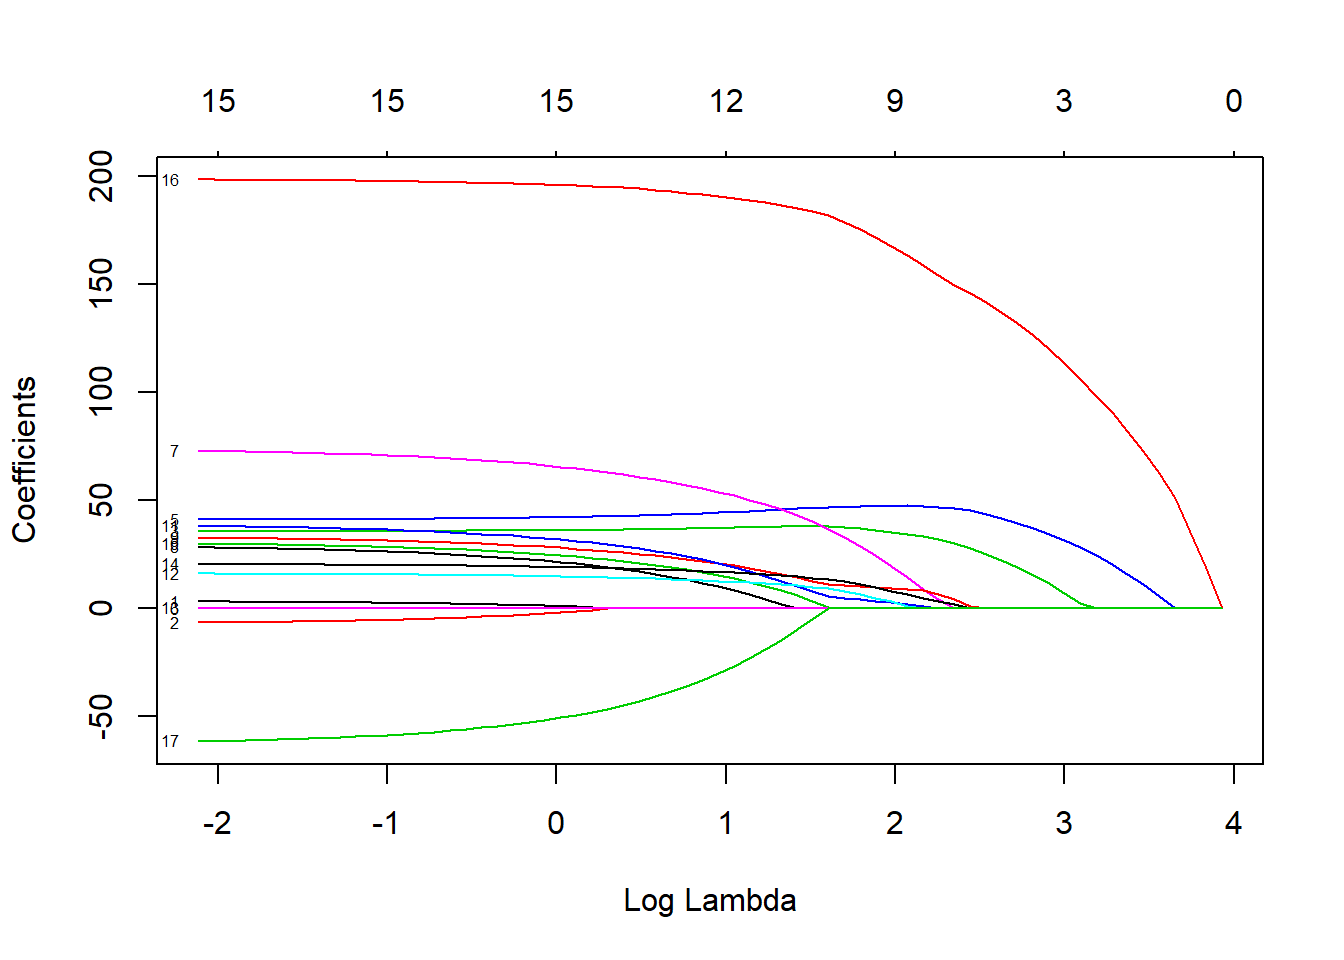
\includegraphics{Airfares_files/figure-latex/unnamed-chunk-17-1.pdf}

\begin{Shaded}
\begin{Highlighting}[]
\CommentTok{\# Cross validation to find value for la}
\NormalTok{cv\_lasso }\OtherTok{=} \FunctionTok{cv.glmnet}\NormalTok{(}\AttributeTok{x =}\NormalTok{ Airfare\_X, }\AttributeTok{y =}\NormalTok{ Airfare\_Y, }\AttributeTok{family =} \StringTok{"gaussian"}\NormalTok{, }\AttributeTok{alpha =} \DecValTok{1}\NormalTok{, }\AttributeTok{nfolds =} \DecValTok{10}\NormalTok{)}
\FunctionTok{plot}\NormalTok{(cv\_lasso)}
\end{Highlighting}
\end{Shaded}

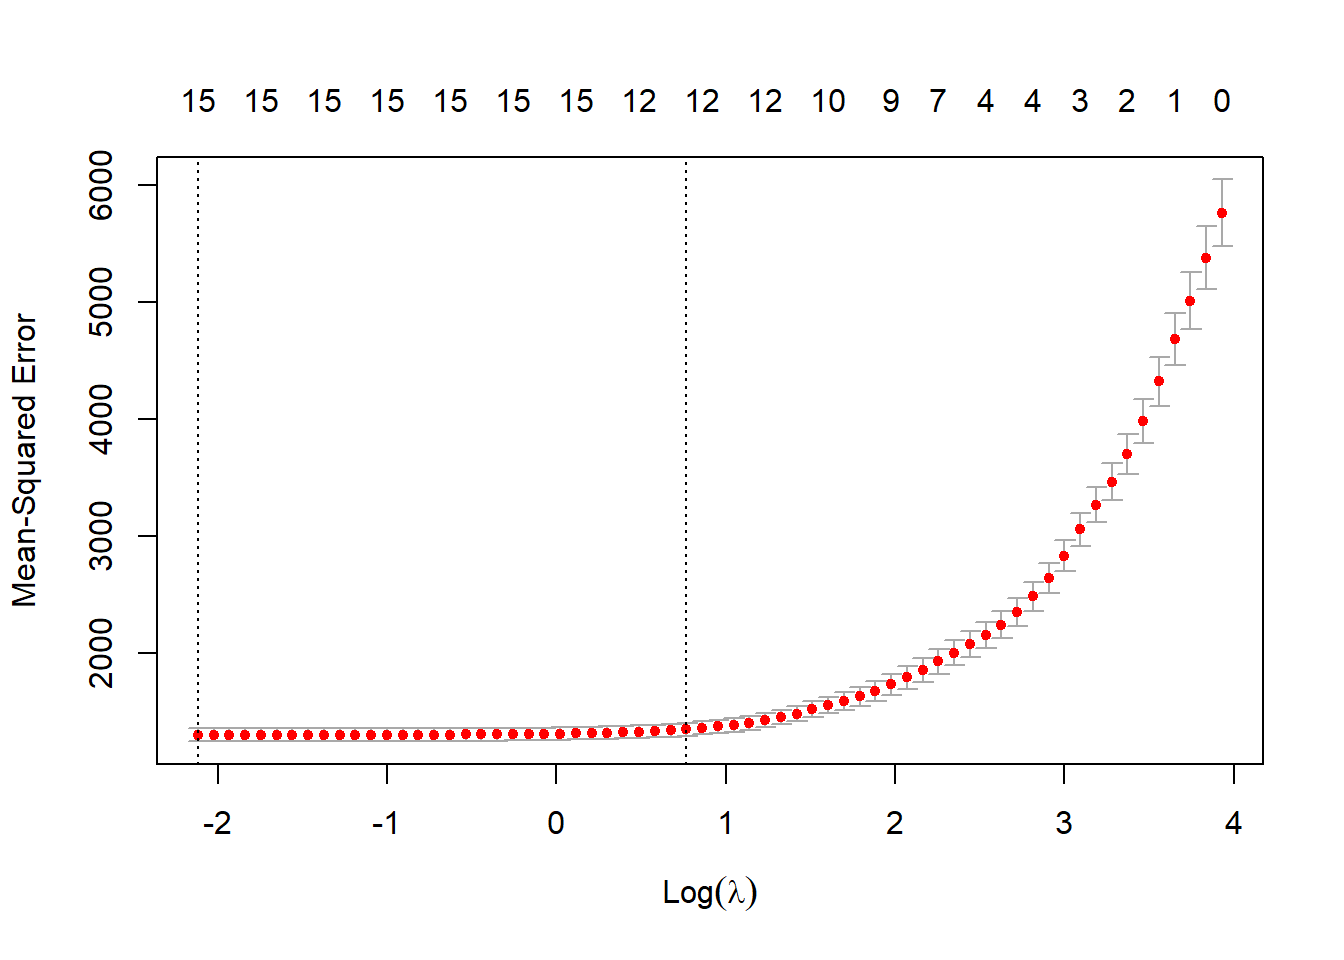
\includegraphics{Airfares_files/figure-latex/unnamed-chunk-18-1.pdf}

\begin{Shaded}
\begin{Highlighting}[]
\CommentTok{\# Predicting LASSO value, taking lambda\textquotesingle{}s minimum value}
\NormalTok{Lasso.Predict }\OtherTok{=} \FunctionTok{predict}\NormalTok{(lasso\_fit,}\AttributeTok{newx =}\NormalTok{ Airfare\_X, }\AttributeTok{s=}\NormalTok{cv\_lasso}\SpecialCharTok{$}\NormalTok{lambda.min)}
\CommentTok{\# Accuracy using the first LASSO method}
\NormalTok{AccuracyLS.min }\OtherTok{=} \FunctionTok{sum}\NormalTok{(}\FunctionTok{abs}\NormalTok{(Lasso.Predict }\SpecialCharTok{{-}}\NormalTok{ Airfare\_Y))}\SpecialCharTok{/}\FunctionTok{length}\NormalTok{(Airfare\_Y) }\CommentTok{\#27.50271}
\CommentTok{\# Predicting LASSO value, taking lambda\textquotesingle{}s standard error of the minimum}
\NormalTok{Lasso.Predict1se }\OtherTok{=} \FunctionTok{predict}\NormalTok{(lasso\_fit, }\AttributeTok{newx =}\NormalTok{ Airfare\_X, }\AttributeTok{s=}\NormalTok{cv\_lasso}\SpecialCharTok{$}\NormalTok{lambda}\FloatTok{.1}\NormalTok{se)}
\CommentTok{\# Accuracy using the second LASSO method}
\NormalTok{AccuracyLS}\FloatTok{.1}\NormalTok{se }\OtherTok{=} \FunctionTok{sum}\NormalTok{(}\FunctionTok{abs}\NormalTok{(Lasso.Predict1se }\SpecialCharTok{{-}}\NormalTok{ Airfare\_Y))}\SpecialCharTok{/}\FunctionTok{length}\NormalTok{(Airfare\_Y) }\CommentTok{\#28.71035}
\end{Highlighting}
\end{Shaded}

SUMMARY

\begin{Shaded}
\begin{Highlighting}[]
\NormalTok{MACHINE\_LEARNING\_MODELS }\OtherTok{=} \FunctionTok{c}\NormalTok{(}\StringTok{"Multiple Linear Regression"}\NormalTok{,}\StringTok{"Decision Tree Model"}\NormalTok{,}\StringTok{"Extreme Gradient Boosting"}\NormalTok{,}\StringTok{"LASSO Regression"}\NormalTok{)}
\NormalTok{ERROR }\OtherTok{=} \FunctionTok{c}\NormalTok{(AccuracyLR,AccuracyDT,AccuracyXgb,AccuracyLS.min)}

\NormalTok{df }\OtherTok{=} \FunctionTok{data.frame}\NormalTok{(MACHINE\_LEARNING\_MODELS,ERROR)}
\NormalTok{df}
\end{Highlighting}
\end{Shaded}

\begin{verbatim}
##      MACHINE_LEARNING_MODELS    ERROR
## 1 Multiple Linear Regression 26.73086
## 2        Decision Tree Model 28.19225
## 3  Extreme Gradient Boosting 48.06455
## 4           LASSO Regression 27.50252
\end{verbatim}


\end{document}
